\chapter{Introduction}
\label{cha:introduction}

The research work that I describe in this dissertation is concerned with the implementation of a Java framework, named \texttt{xmlet}, which allows the automatic generation of a Java \textit{fluent interface}\cite{fluentinterface} recreating a \ac{DSL}\cite{dsl} specified by an \ac{XML} schema. The approach described in this work can be further applied to any other strongly typed environment. As an example of \ac{DSL} generation we used \texttt{xmlet} to automatically create a Java \ac{DSL} for \ac{HTML}5, named \textit{HtmlFlow}\cite{htmlflow}. A \ac{DSL} for \ac{HTML} can be used as a type safe template engine that results in an improvement in the numerous existing \textit{template engines}. Furthermore, \textit{HtmlFlow} outperforms state-of-the-art Java \textit{template engines}, namely Rocker\cite{rocker}, Pebble\cite{pebble}, Trimou\cite{trimou} or Mustache\cite{mustache}, in some of the more challenging benchmarks such as \textit{template-benchmarks}\cite{templatebenchmark} and \textit{spring-comparing-template-engines}\cite{springbenchmark}.

\section{Introduction to Domain Specific Languages}

\lstdefinestyle{dynamicviewsex}{
  moredelim=**[is][\color{green}]{@}{@}, 
  moredelim=**[is][\color{blue}]{|}{|},
}

High-level programming languages such as Java, C\# and JavaScript and others were created with the objective of being abstract, in the sense that they do not compromise with any specific problem. Using these programming languages is usually enough to solve most problems but in some specific situations solving problems using exclusively those languages is counter-productive. A good example of that counter-productivity is thinking about regular expressions. In the Martin Fowler \ac{DSL} book\cite{dslbook} we can find the regular expression presented in Listing \ref{lst:regexexpression}.

\bigskip

\begin{minipage}{\linewidth}
\begin{lstlisting}[caption={Regular Expression Example}, label={lst:regexexpression}, style=dynamicviewsex]
|\d{3}-\d{3}-\d{4}|
\end{lstlisting}
\end{minipage} 

\noindent
Looking at the expression of Listing \ref{lst:regexexpression} the programmer understands that it matches a \texttt{String} similar to \texttt{123-321-1234}. Even though the regular expression syntax might be hard to understand at first glance, after a while it may become understandable. It may be easier to use and manipulate by experts than implementing the same set of rules to verify a \texttt{String} using control instructions such as \texttt{if/else} and \texttt{String} operations. It also makes the communication between experts easier when dealing with this concrete problem because there is a standard syntax with well-known rules. Regular expressions are just one of the many examples that show that creating an explicit language to deal with a very specific problem simplifies it. Other examples of \ac{DSL}s are languages such as \ac{SQL}\cite{sql}, \texttt{Apache Ant}\cite{ant} or \texttt{make}\cite{make}. 

\noindent
\ac{DSL}s can be divided in two types: external or internal. External \ac{DSL}s are languages created without any affiliations to a concrete programming language. An example of an external \ac{DSL} is the regular expressions \ac{DSL}, since it defines its own syntax without any dependency of programming languages. On the other hand an internal \ac{DSL} is defined within a programming language, such as Java. An example of an internal \ac{DSL} is the JMock\cite{jmock} which is a Java library that provides tools for test-driven development as shown in Listing \ref{lst:jmock}. 

\bigskip

\lstset{language=java, morekeywords={GreetingTime, mock, setGreetingTime, checking, Expectations, one, getGreeting, will, returnValue}}

\begin{minipage}{\linewidth}
\begin{lstlisting}[caption={JMock Use Example}, label={lst:jmock}]
final GreetingTime gt = context.mock(GreetingTime.class);
Greeting g = new Greeting();
g.setGreetingTime(gt);

context.checking(new Expectations(){{
	one(gt).getGreeting(); will(returnValue("Good afternoon"));
}});
\end{lstlisting}
\end{minipage} 

\noindent
In Listing \ref{lst:jmock} we can see that JMock uses a \ac{DSL} to create expectations. In the concrete example it obtains the value of a \texttt{Greeting} and asserts if the value \texttt{will} be \texttt{Good afternoon}. In this case the semantics of the methods used by JMock is meant to make it easier for the programmer to understand the tests that are being performed.

\noindent
Internal \ac{DSL}s can also be referred to as embedded \ac{DSL}s since they are embedded in the programming language that where they are used. Another common term for an internal \ac{DSL} is \textit{fluent interface} or \textit{fluent \ac{API}}. The term fluent is inspired by the fluent way that the \ac{DSL} usage can be read, which is close to a natural language.

\noindent
Concluding, there are some advantages on internal \ac{DSL}s over external \ac{DSL}s, namely: a single compiler, removal of language heterogeneity and in some situations, performance improvements and overall a less complex solution.

\noindent
From a simple point of view, one of the main goals of this research work is to propose an approach and develop a platform, i.e. \texttt{xmlet}, which enables the conversion of an \ac{XML} based external \ac{DSL} into an internal \ac{DSL}. One of the requirements of this approach is that the external \ac{DSL} rules must be defined by an \ac{XSD} document. Thus, on one hand we have a \ac{XSD} document that defines a set of elements, attributes and rules that together define their own \ac{XML} language. From a Java environment point of view this \ac{XML} language is qualified as an external \ac{DSL} since it is defined in \ac{XML} which is a markup language that does not depend of the Java programming language. All the information present in the \ac{XSD} document is used to generate a Java \textit{fluent interface}, which, in this case, is an internal \ac{DSL} since it uses the Java syntax to define the \ac{DSL}. 

\noindent
Using this approach we are going to generate a \textit{fluent interface} for the \ac{HTML}5 language, based on its \ac{XSD} document. The result of our approach is the automatic code generation of Java classes and interfaces that will reflect all the information present in the \ac{XSD} document. When we analyze the end result of this work, what we achieve is a Java interface to manipulate a \ac{DSL}, in this case \ac{HTML}, which can be used for anything related with \ac{HTML} manipulation with the upside of having the guarantee that the rules of that language are verified. One of those usages is writing well-formed \ac{HTML} documents and defining \textit{dynamic views} that will be filled with information received in runtime. An example of a static view is presented in Listing \ref{lst:staticview}.

\bigskip

\lstset{language=java, morekeywords={html, body, h1, text, StaticHtml}}

\begin{minipage}{\linewidth}
\begin{lstlisting}[caption={Static View Example with HtmlFlow}, label={lst:staticview}, literate={º}{\textdegree}1]
private static void staticView(StaticHtml view){
    view.html()
            .body()
                .h1()
                    .text("This is a static view h1 element.")
                .º()
            .º()
        .º();
}
\end{lstlisting}
\end{minipage} 

\noindent
The static view of Listing \ref{lst:staticview} shows how an internal \ac{DSL} guarantees the rules of the language by using Java to enforce them. In this concrete example we can see that the logic of element organization of the \ac{HTML} language is translated to Java methods, ensuring, for example, that the \texttt{html} element can only contain either \texttt{head} or \texttt{body} element as children.

\section{Template Engines}
\label{sec:templateengines}

\texttt{Template engines} are solutions that use views, more specifically \textit{dynamic views}, to build a documents. A view is the output representation of information used to build the user interface of an application. Regarding web applications the view may be defined using the \ac{HTML} language.

\subsection{Dynamic Views}

In this context, a \textit{dynamic view} is a template with two distinct components, as shown in Listing \ref{lst:dynamicstudentinfo}, a {\color{blue}static component}, represented in blue, which defines the structure of the document and a {\color{green}dynamic component}, represented in green, which is represented by \textit{placeholders} that are replaced by information received at runtime. A simple example of a \textit{dynamic view} can be an \ac{HTML} template with the information of a given \texttt{Student}, as shown in Listing \ref{lst:dynamicstudentinfo}. 

\bigskip

\begin{minipage}{\linewidth}
\begin{lstlisting}[caption={HTML Template of Student information in Mustache idiom}, label={lst:dynamicstudentinfo}, style=dynamicviewsex]
|<html>
    <body>
        <ul>|
        @{{#student}}
            <li>
                {{name}}
            </li>
            <li>
                {{number}}
            </li>
        {{/student}}@
|        </ul>
    </body>
</html>|
\end{lstlisting}
\end{minipage} 

\noindent
To generate the resulting \ac{HTML} page from the template of Listing \ref{lst:dynamicstudentinfo} we need external input, received at runtime, to resolve the dynamic component of the view. In the previous example, Listing \ref{lst:dynamicstudentinfo}, the view needs to receive a value for the variable named \texttt{\char`\{\char`\{student\char`\}\char`\}}. The type that the \texttt{student} variable represents should be a type that contains two fields, a \texttt{number} and a \texttt{name} field. An example of an object with that characteristics is presented in Figure \ref{img:studentclass}.

\begin{figure}[H]
	\centering
	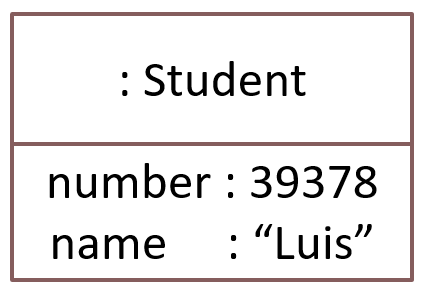
\includegraphics[width=0.25\textwidth]{student_class}
	\caption{Student Object}
	\label{img:studentclass}
\end{figure}

\noindent
After the template in Listing \ref{lst:dynamicstudentinfo} receives the \textit{context object} presented in Figure \ref{img:studentclass} the resulting \ac{HTML} document is as presented in Listing \ref{lst:dynamicstudentinfocomplete}.

\bigskip

\lstset{language=html}

\begin{minipage}{\linewidth}
\begin{lstlisting}[caption={HTML Document with Student information}, label={lst:dynamicstudentinfocomplete}]
<html>
    <body>
        <ul>
            <li>
                Luis
            </li>
            <li>
                39378
            </li>
        </ul>
    </body>
</html>
\end{lstlisting}
\end{minipage} 

\textit{Template engines} are responsible for generating an \ac{HTML} document based on a template. \textit{Template engines} are the most common method to manipulate \textit{dynamic views}. \textit{Template engines} are responsible for performing the combination between the \textit{dynamic view}, also named \textit{template}, and a data model object, known as \textit{context object}, which contains all the information required to generate the final document. The example depicted in Figure \ref{img:templateengineprocess} shows the combination of a template document with a context object, which is an instance of \texttt{Student}.

\begin{figure}[H]
	\centering
	
\includegraphics[width=1\textwidth]{template_engines}
	\caption{Template Engine Process which combines a Template Document with a Context Object}
	\label{img:templateengineprocess}
\end{figure}

\noindent
Since the Web appearance there is a wide consensus around the use of \textit{template engines} to build dynamic \ac{HTML} documents. From the vast list of existing web template engines\cite{listtemplateengines} all of them share the same approach based on a text template file. The \textit{template engine} scope is also wide, even that they are mostly associated with Web, they are also widely used to generate other types of documents such as emails and reports. 

\subsection{Handicaps}
\label{sec:templateengineshandicaps}

Although there is a wide consensus in the use of \textit{template engines}, this approach still has some handicaps, which we will further analyze.

\begin{itemize}
	\item Safety and Type Check - There are no validations of the language used in the templates nor the dynamic information. This can result in documents that do not follow the language rules.
	\item Performance - This aspect can be divided in two, one regarding the text files that are used as templates which have to be loaded and therefore slow the overall performance of the application and the heavy usage of \texttt{String} operations which are inherently slow.
	\item Flexibility - The syntax provided by the \textit{template engines} is sometimes very limited and restricts the operations that can be performed in the template files to few control flow instructions such as \texttt{if/else} operations and \texttt{for} operation to loop data.
	\item Complexity - It introduces one more syntax in the programming environment. For example a Java application using the Mustache\cite{mustache} \textit{template engine} forces the programmer to use three distinct languages: Java, the Mustache syntax in the template file and the \ac{HTML} language.
\end{itemize}

\section{Thesis Statement}
\label{sec:thesisstatement}

This dissertation thesis is that it is possible to reduce the problems that exist within the use of \textit{template engine} solutions. To suppress these handicaps we propose the creation of a process that automatizes the generation of \ac{DSL}s based on a existing \ac{DSL} specified by one \ac{XSD} document. This process is implemented by the \texttt{xmlet} platform, which allows the automatic generation of a strongly typed and fluent interface for a \ac{DSL} based on the rules expressed in the \ac{XSD} document of that respective language, such as \ac{HTML}. The resulting \ac{DSL} addresses the handicaps of the \texttt{template engines} in the following way:

\begin{itemize}
	\item Safety and Type Check - The generated Java \ac{DSL} will guarantee the implementation of the language rules defined in the \ac{XSD} file by reflecting those restrictions in the generated \texttt{fluent interface}.
	\item Performance - Text templates files are replaced by pure Java functions, according to my approach a template is a first-class function.
	\item Flexibility - The syntax to perform operations on templates is replaced to the Java syntax without any restriction to the use of all its features.
	\item Complexity - It replaces the heterogeneity of using three programming languages, i.e. Java, \ac{HTML} and the \texttt{template engine} specific idiom, with the use of a single programming language.
\end{itemize}

\noindent
A brief view of the generated \textit{fluent interface} is presented in Listing \ref{lst:xmletdynamicstudentinfo}, which shows how the previous example in the Mustache idiom, i.e. Listing \ref{lst:dynamicstudentinfo}, will be recreated with the \texttt{xmlet} solution. The specific details on how the code presented in this example works will be provided in Chapter \ref{cha:solution}.

\bigskip

\lstset{language=java, morekeywords={String, DynamicHtml, view, render, CurrentClass, studentView, Student, html, body, ul, li, dynamic, text, getName, getNumber}}

\begin{minipage}{\linewidth}
\begin{lstlisting}[caption={Xmlet Template with Student information}, label={lst:xmletdynamicstudentinfo}, literate={º}{\textdegree}1]
String document = DynamicHtml.view(CurrentClass::studentView)
                             .render(new Student("Luis", 39378));

static void studentView(DynamicHtml<Student> view, Student student){
    view.html()
          .body()
            .ul()
              .li().dynamic(li -> li.text(student.getName())).º()
              .li().dynamic(li -> li.text(student.getNumber())).º()
            .º()
          .º()
        .º();   
}
\end{lstlisting}
\end{minipage} 

\noindent
To implement the \texttt{xmlet} process we created three distinct components:

\begin{itemize}
	\item XsdParser - Which parses the \ac{DSL} described in a \ac{XSD} document in order to extract information needed to generate the internal Java \ac{DSL}.
	\item XsdAsm - Which uses XsdParser to gather the required information to generate the internal Java \ac{DSL}.
	\item HtmlApi - A concrete Java \ac{DSL} for the \ac{HTML}5 language generated by XsdAsm using the \ac{HTML}5 \ac{XSD} document.
\end{itemize}

\noindent
The use case for this dissertation will be the \ac{HTML} language but the process is designed to support any domain language that has its definition in the \ac{XSD} syntax. This means that any \ac{XML} language should be supported as long as it has its set of rules properly defined in a \ac{XSD} file. To show that this solution is viable with other \ac{XSD} files we used another \ac{XSD} file that detailed the rules of the \ac{XML} syntax used to generated Android\cite{android} visual layouts.

\section{Document Organization}

This document will be separated in six distinct chapters. The first chapter, this one, introduces the concept that will be explored in this dissertation. The second chapter introduces the motivation for this dissertation. The third chapter presents existent technology that is relevant to this solution. The fourth chapter explains in detail the different components of the suggested solution. The fifth chapter approaches the deployment, testing and compares the \texttt{xmlet} solution to other existing solutions. The sixth and last chapter of this document contains some final remarks and description of future work.